\documentclass{beamer}
\usetheme{Madrid}
\usepackage[normalem]{ulem}

\begin{document}

\title{Team D Project Plan}
\author[CK, TW, ES, AM, JW, \& FS]{Cory Kolbeck, Tony Wooster, Erik Swanson, Adrian Miranda, Justin Wagner, and Federico Saldarini}
\institute[PSU]{
  Portland State University\\
  Department of Computer Science\\
  Portland, Oregon\\
}

\begin{frame}
  \titlepage
\end{frame}

\begin{frame}{Overview and Deliverables}
  \begin{center}{
      \large
      \textbf{We are to implement client libraries to provide asynchronous communication with a Burrow message queue server.}

      \vspace{1cm}
      
      The code for these libraries will reside on Github, and the sponsor will link to them from the main Burrow site. 
      Documentation will reside on the main Burrow website. 
    }
  \end{center}
\end{frame}

\begin{frame}{Assumptions}

  \begin{itemize}
  \item The code will be maintained by the OpenStack community
  \item The code will continue to reside on Github, or possibly be moved to launchpad
  \item Documentation will be hosted on burrow.openstack.org
  \item Authentication is outside the scope of this project
  \end{itemize}

\end{frame}

\begin{frame}{Restraints}

  \begin{itemize}
  \item Project will be distributed under the Apache2 license, and any libraries used must be compatible.
  \item All calls in to our library must be nonblocking.
  \item Maven will be used for Java builds.
  \item The Pandora autoconf macro set will be used for C builds.
  \item Minimal dependence on external libraries.
  \end{itemize}

\end{frame}

\begin{frame}{Plan Overview}
  The team will be split into two teams of three.
  Erik, Justin, and Cory will create a library in Java.
  Tony, Fede and Adrian will create a library in C.

  \begin{enumerate}
  \item \sout{Meet with Eric Day to discuss project details}
  \item \sout{Decide on target languages}
  \item \sout{Create skeleton projects} and integrate them with burrow continuous integration infrastructure
  \item Create blocking memory backends
  \item Research and choose JSON and HTTP libraries
  \item Create blocking memory backend 
  \item Research asynchronous I/O
  \item \sout{Choose language appropriate callback mechanisms}
  \item Write asynchronous memory backend
  \item Write asynchronous http backend
  \item Write functional tests
  \item \textit{Time Allowing} Write small projects which use our libraries in interesting ways.
  \end{enumerate}
\end{frame}

\begin{frame}{C Gantt Chart}
  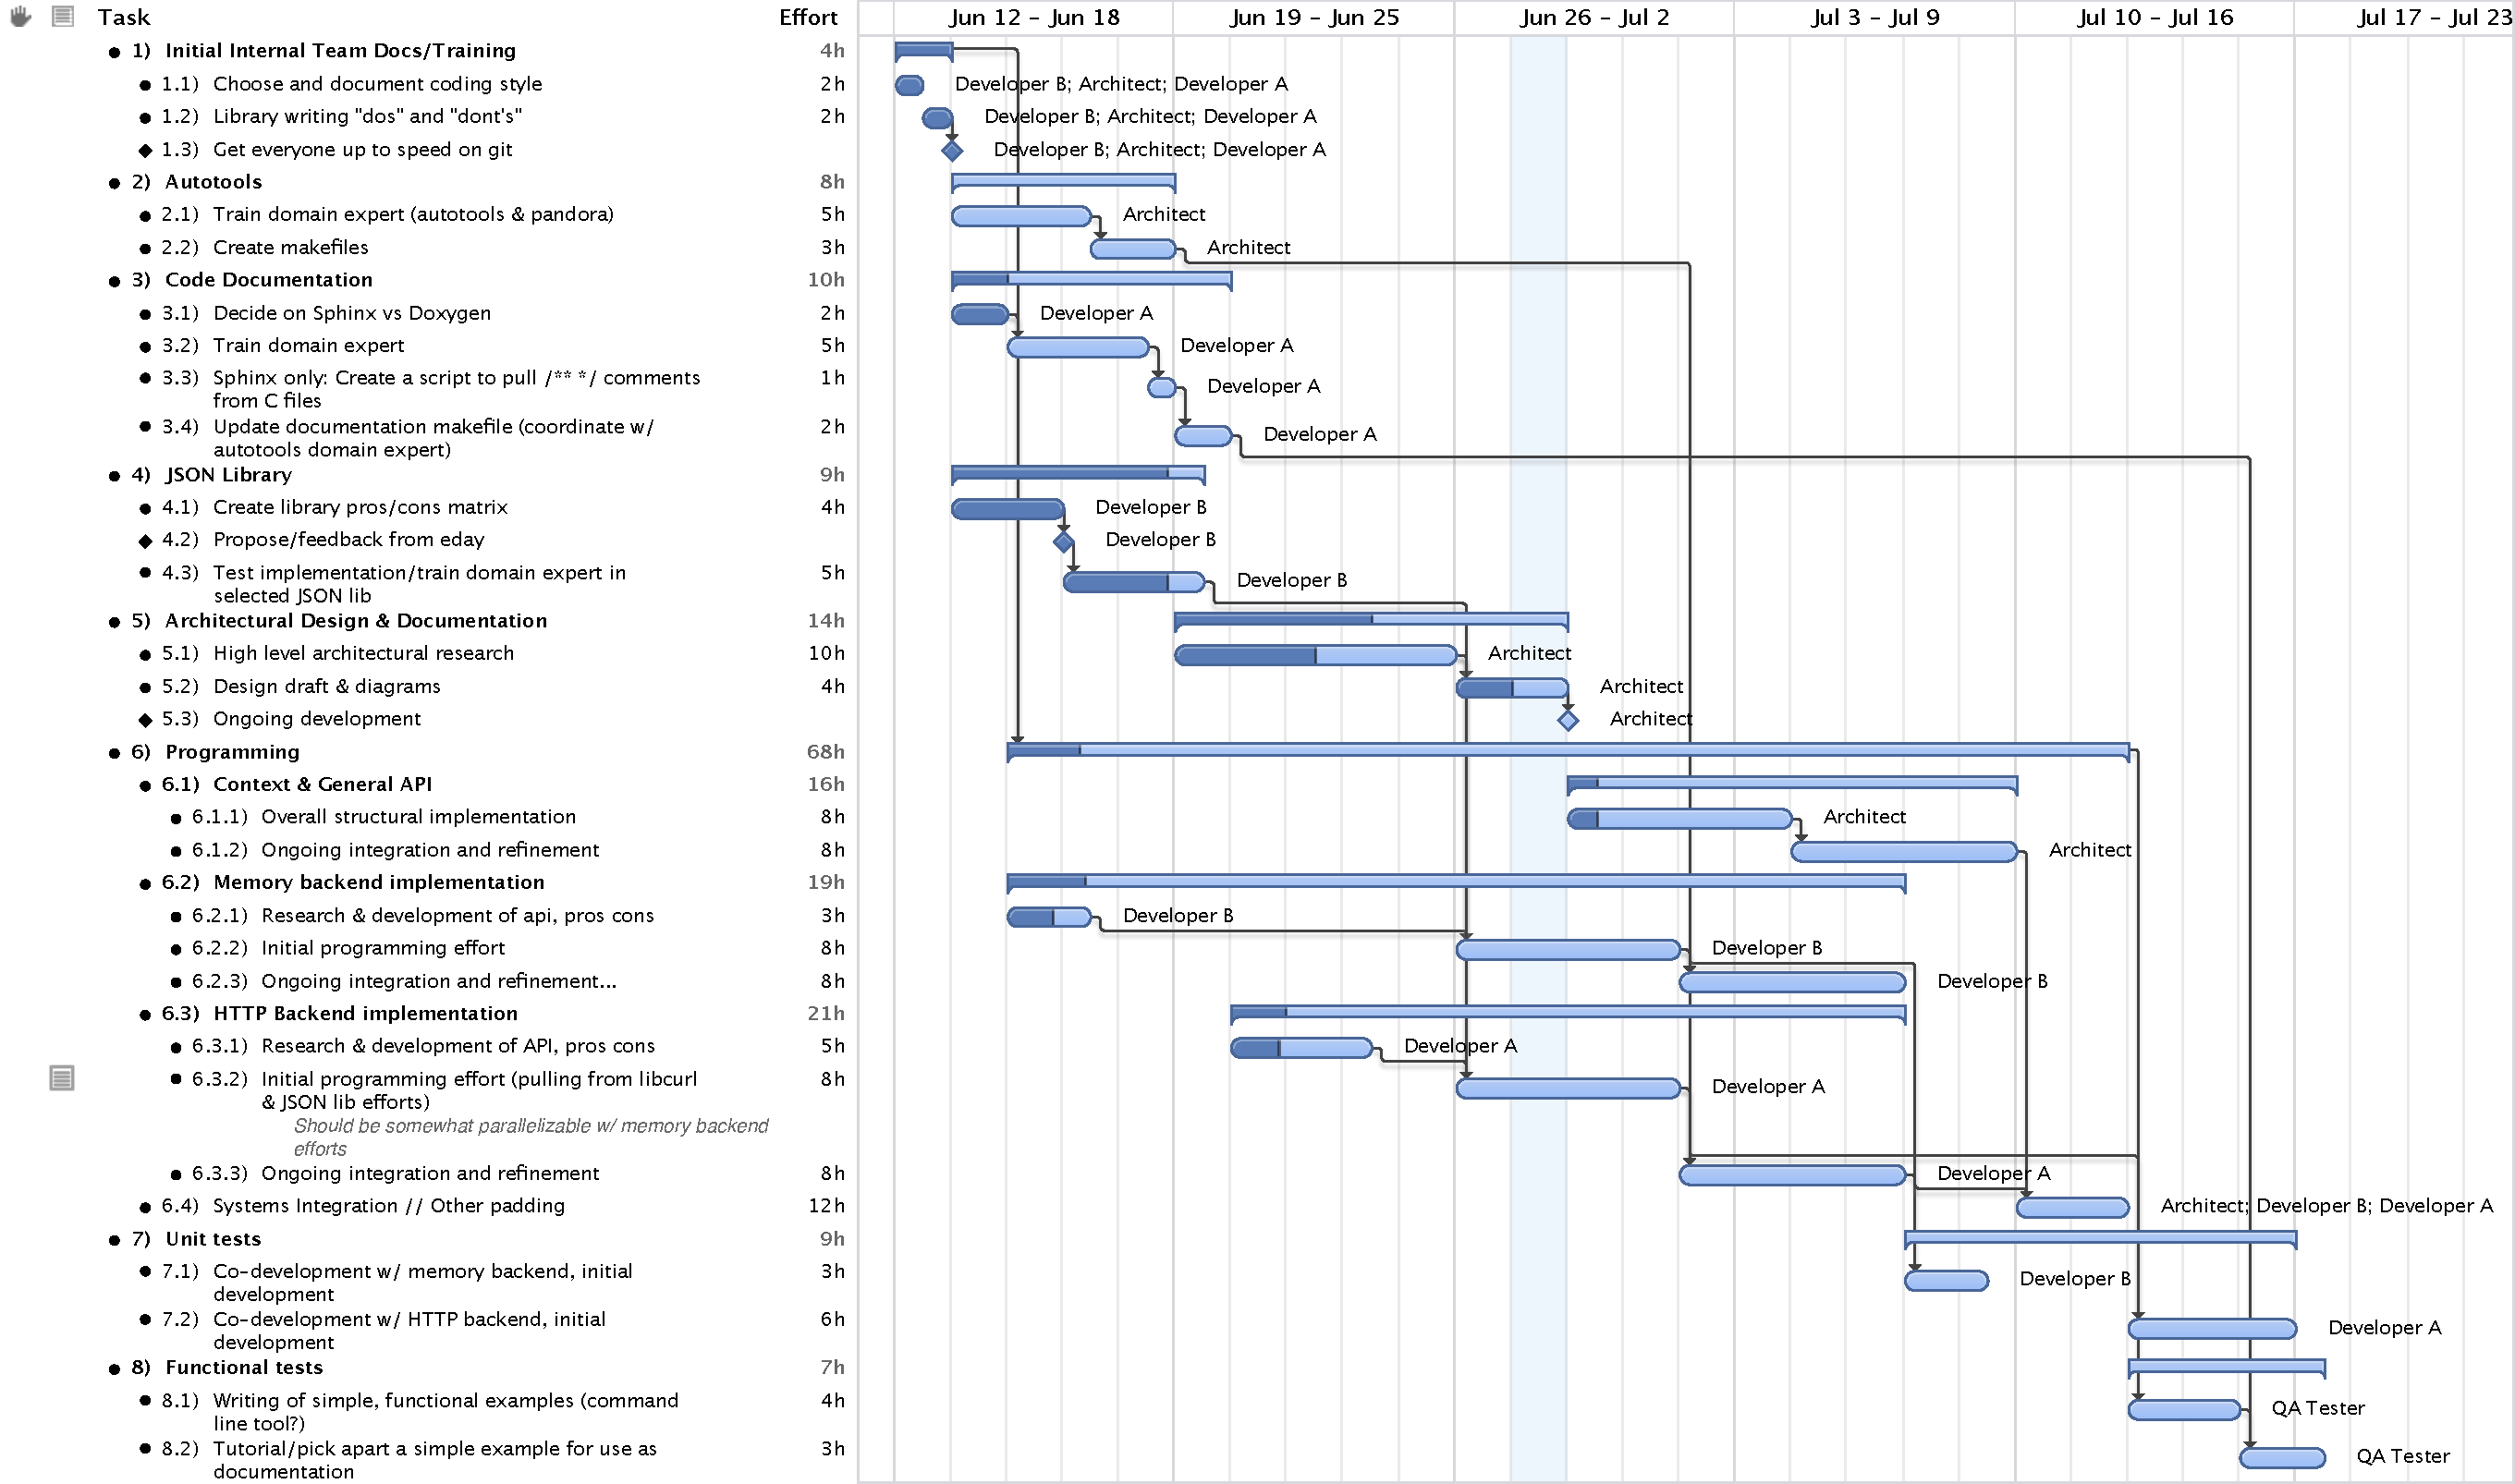
\includegraphics[width=0.95\linewidth]{C-Gantt.pdf}
\end{frame}

\begin{frame}{Java Gantt Chart}
  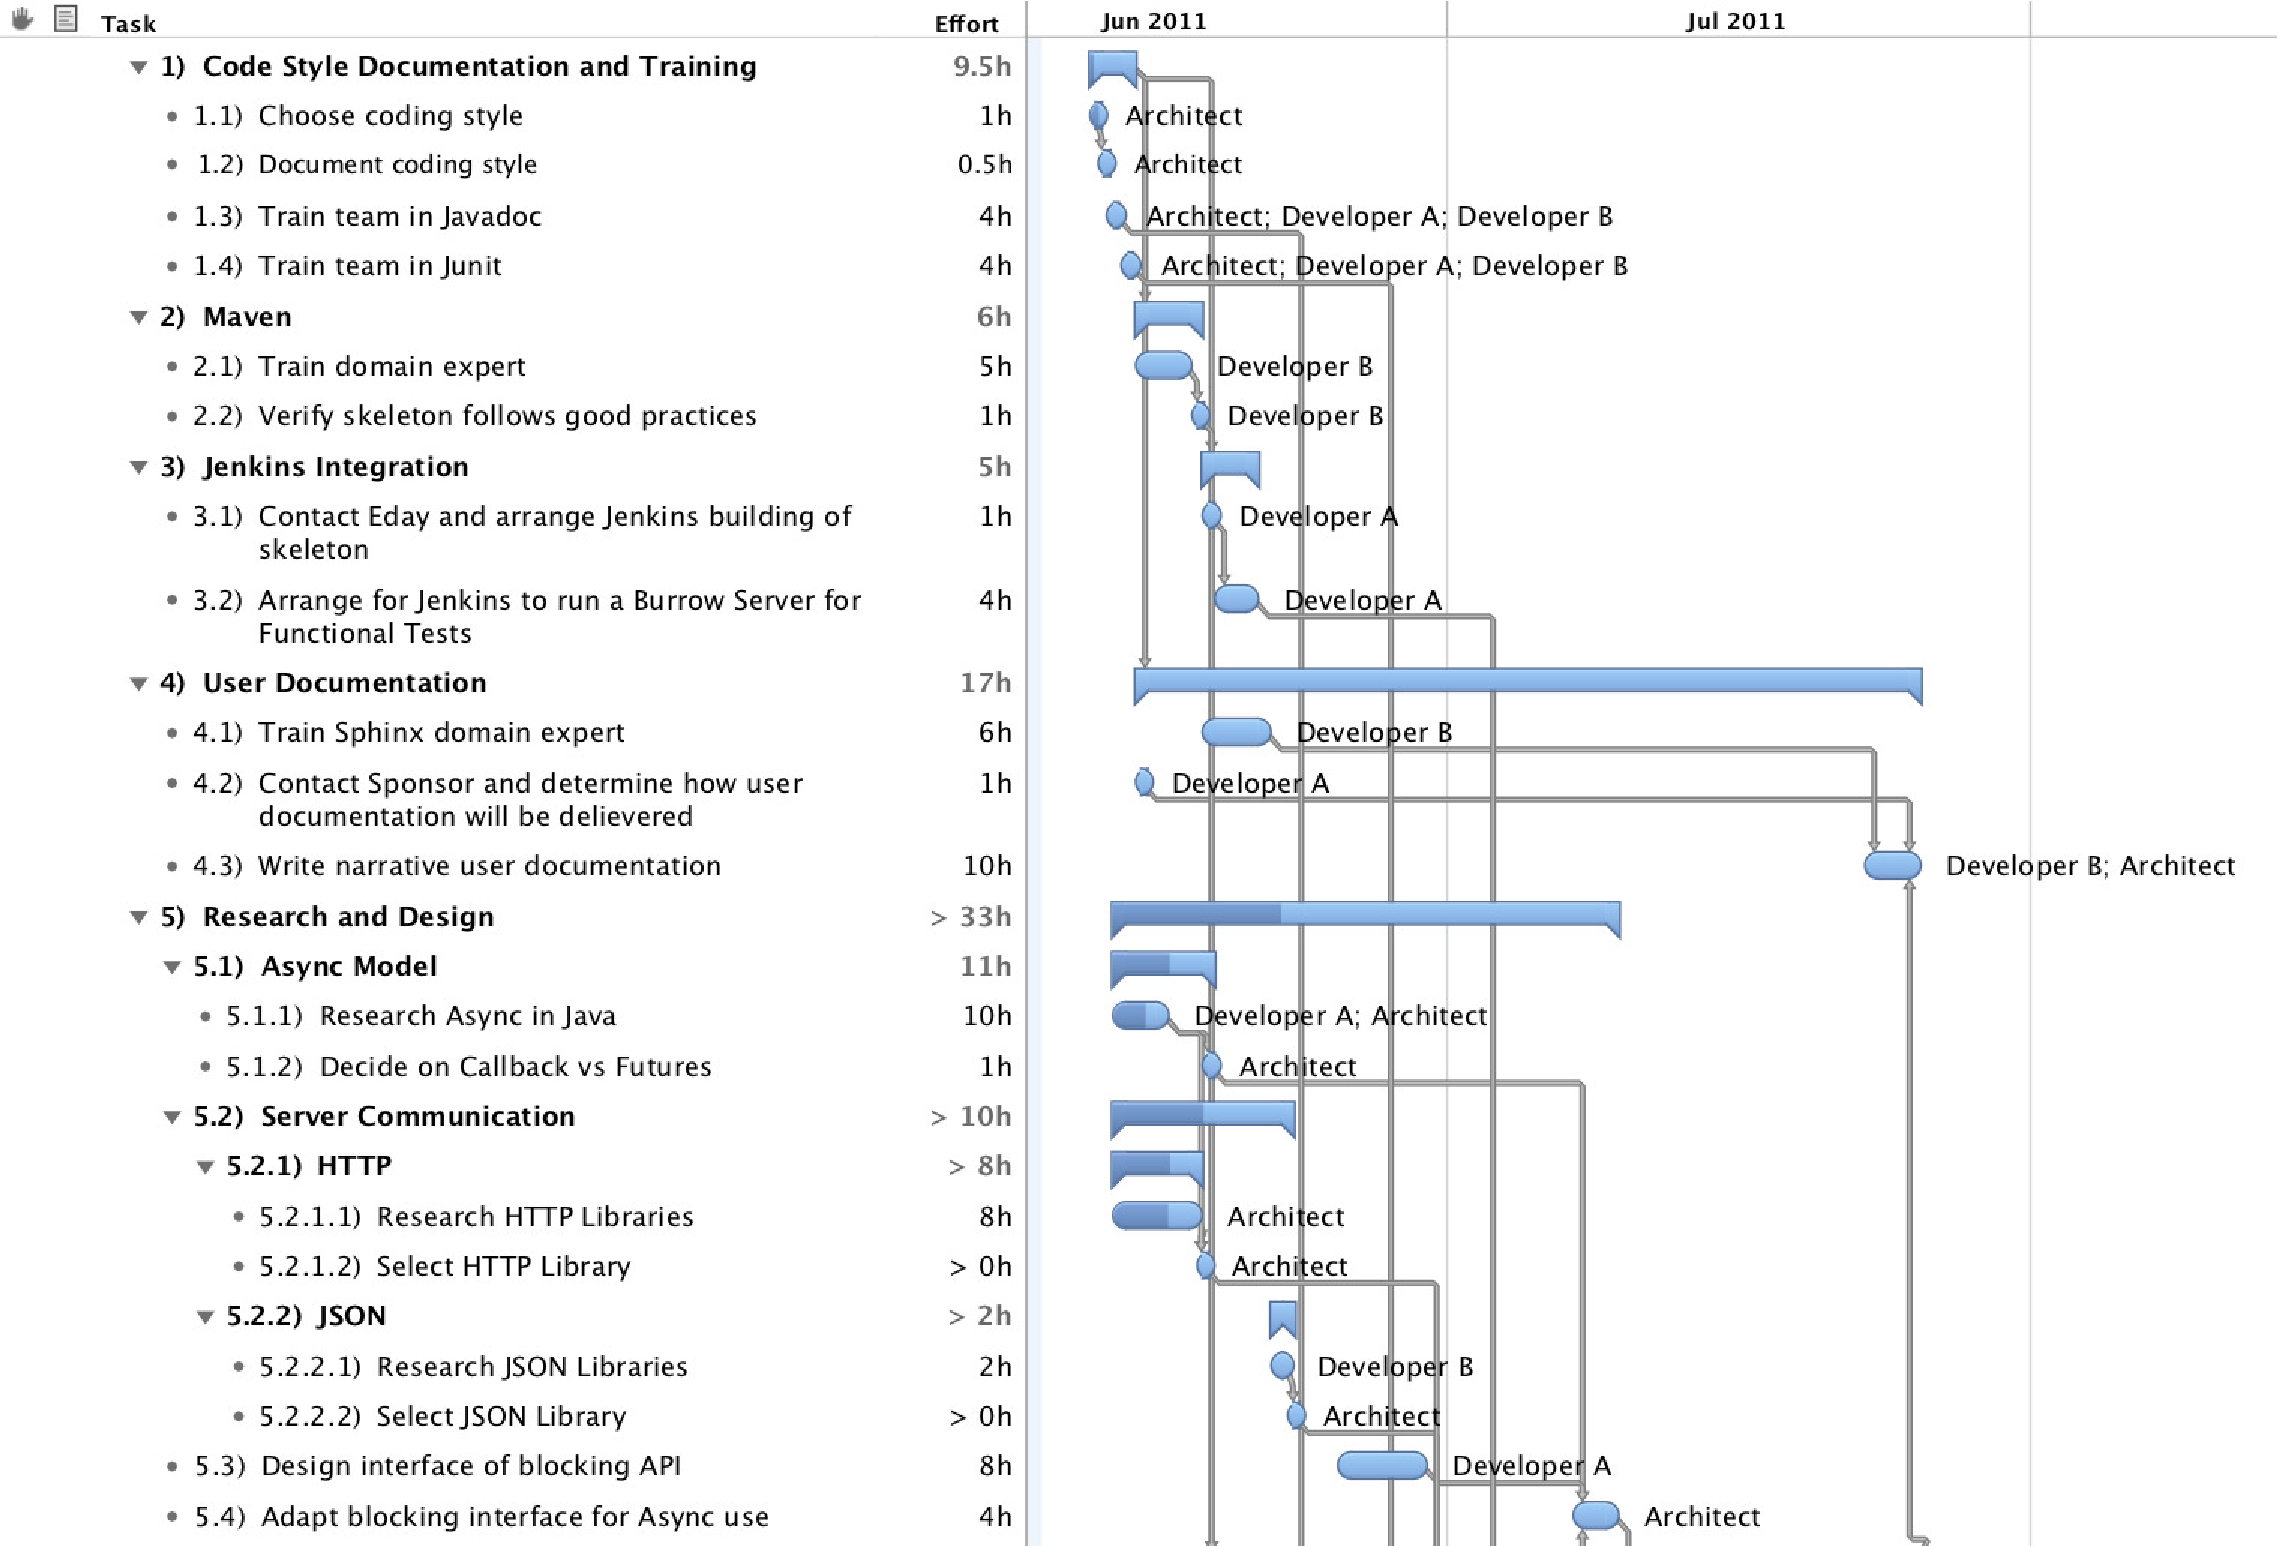
\includegraphics[width=0.95\linewidth]{Java-Gantt-P1.pdf}
\end{frame}

\begin{frame}{Java Gantt Chart}
  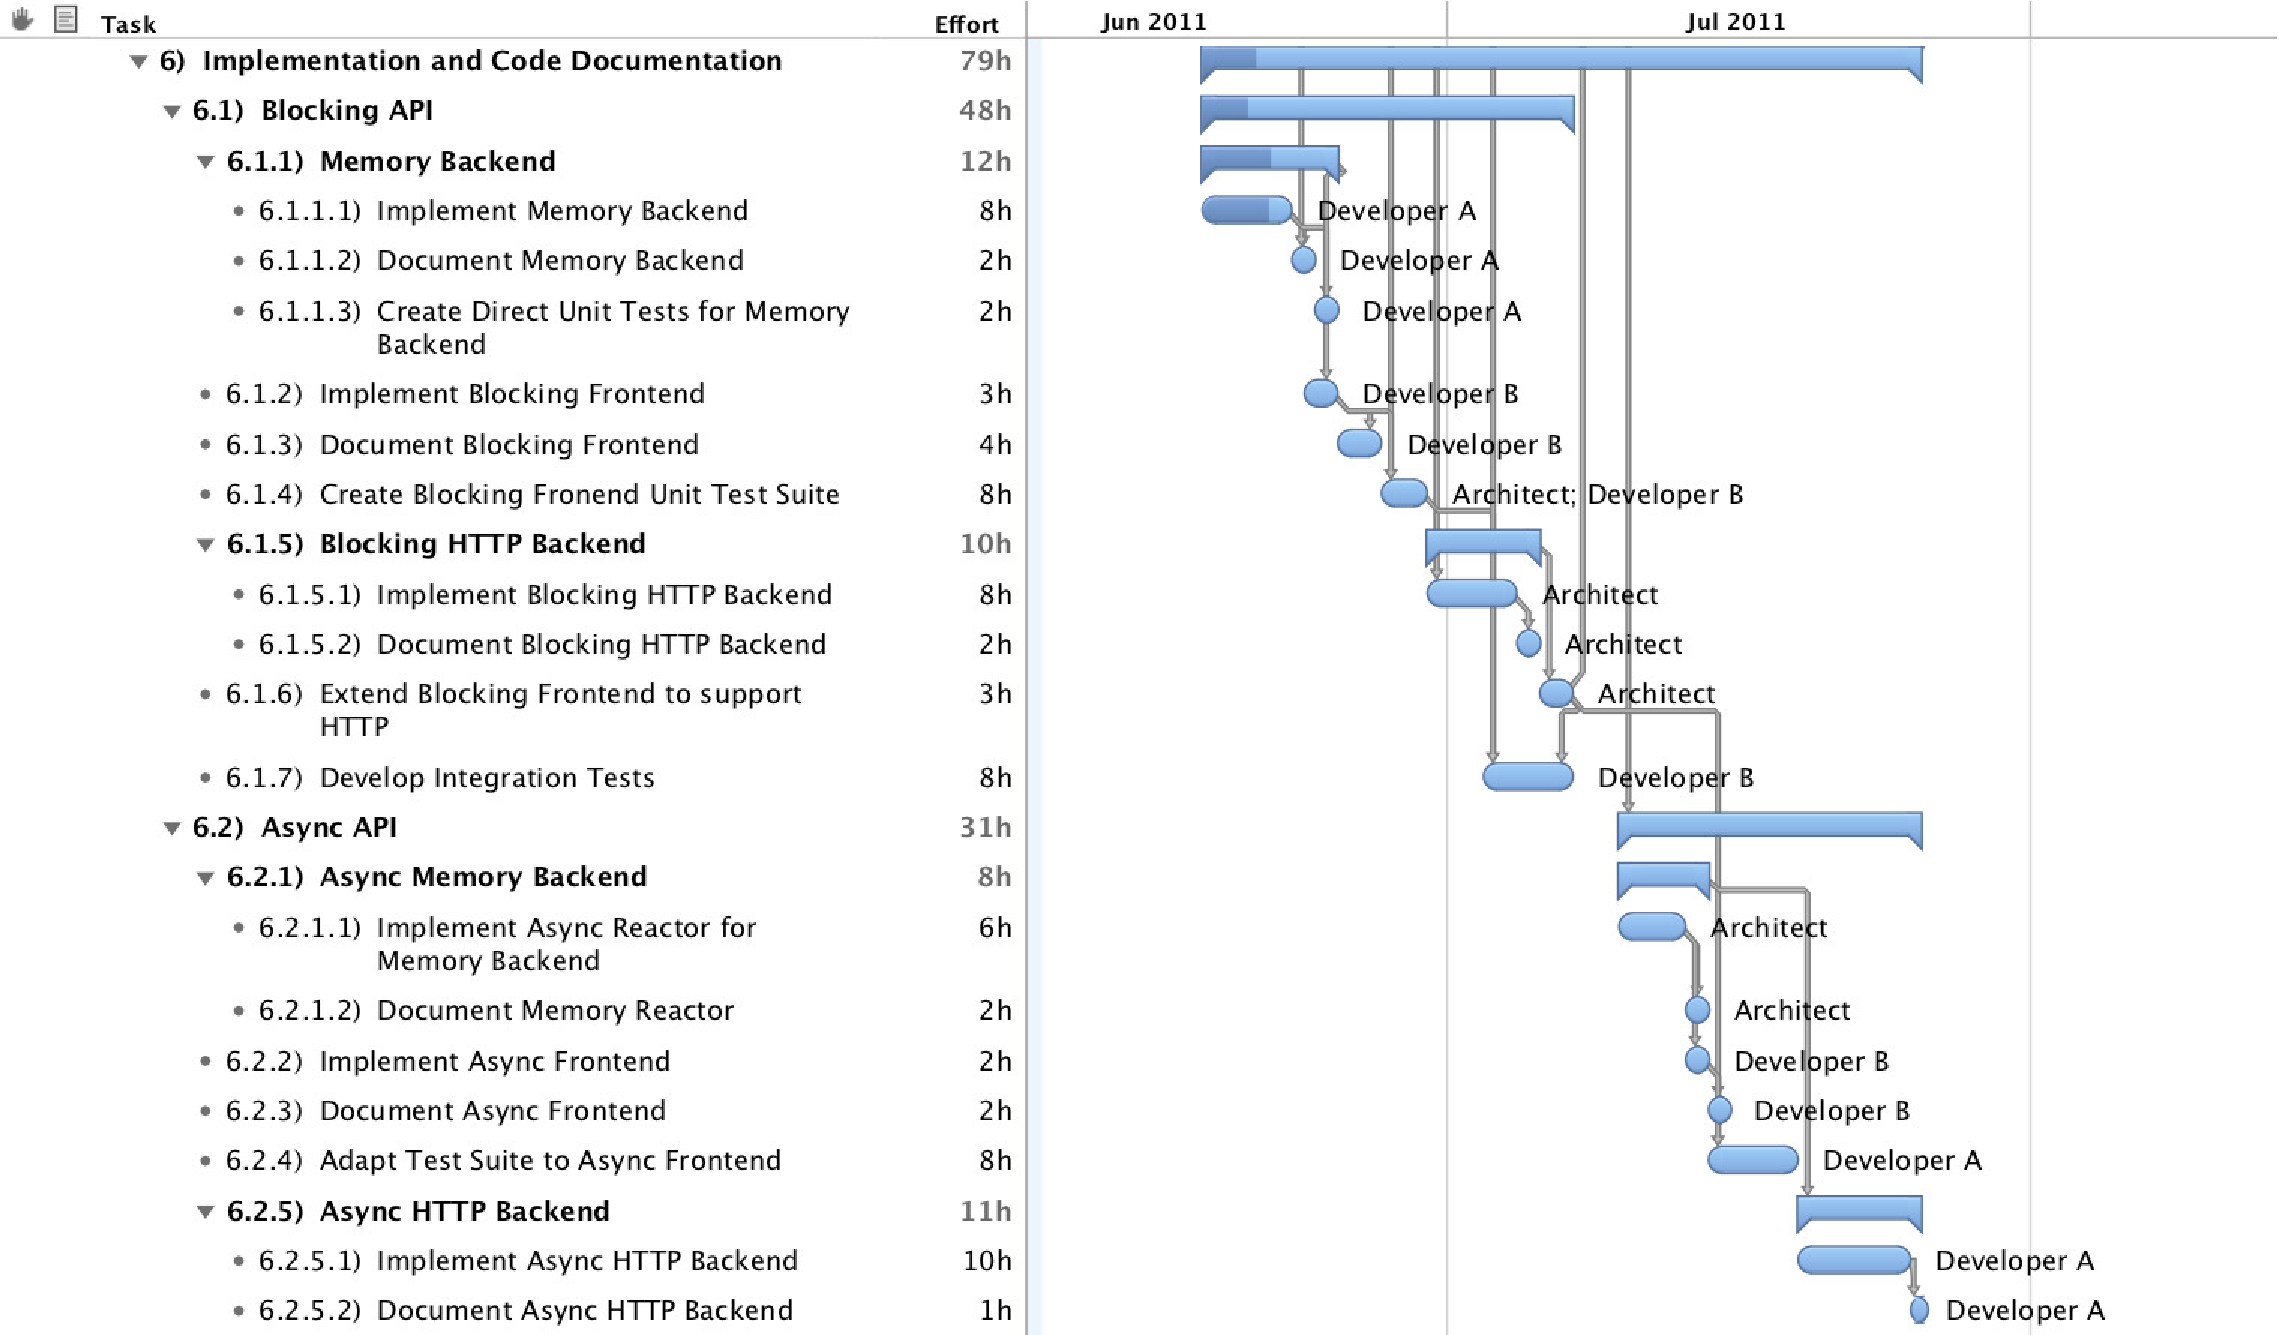
\includegraphics[width=0.95\linewidth]{Java-Gantt-P2.pdf}
\end{frame}

\begin{frame}{Calendar}
  \begin{center}
    \begin{tabular}{|c|c|}
      \hline
      \emph{Week of} & \emph{Deliverable}\\ \hline \hline
      Jun 05 & Project Plan, Architecture Overview\\ \hline
      Jun 12 & \\ \hline
      Jun 19 & \\ \hline
      Jun 26 & Blocking Memory Backend\\ \hline
      Jul 03 & Blocking HTTP Backend\\ \hline
      Jul 10 & \\ \hline
      Jul 17 & Async Memory Backend\\ \hline
      Jul 24 & Async HTTP Backend\\ \hline
      Jul 31 & Narrative Documentation, Sponsor Delivery\\\hline
      Aug 08 & Final Presentation\\ \hline
    \end{tabular}
    \end{center}
\end{frame}

\begin{frame}{Meetings and Reviews}
  \begin{itemize}
  \item In person meetings with sponsor every 1-2 weeks.
  \item IRC consultation as needed.
  \item Reviews at milestones as previously noted.
  \end{itemize}
\end{frame}

\begin{frame}{Resource Identification - Time}
  \begin{center}
    \begin{tabular}{|c|c|}
      \hline
      \emph{Name} & \emph{Available Hours/Week}\\ \hline \hline
      Justin & 8-10\\ \hline
      Adrian & 8-10\\ \hline
      Tony & 8-10\\ \hline
      Erik & 10-15\\ \hline
      Federico & 10+\\ \hline
      Cory & 10-15 \\
      \hline
    \end{tabular}
  \end{center}
\end{frame}

\begin{frame}{Resource Identification - Expertise}
  \begin{center}
    \begin{tabular}{|r|l|}
      \hline
      \emph{Name} & \emph{Expertise}\\ \hline \hline
      Justin & -\\ \hline
      Adrian & -\\ \hline
      Tony & REST \\ \hline
      Erik & REST \\ \hline
      Federico & -\\ \hline
      Cory & Parallel architecture, Basic Git \\ \hline
      Eric & Async I/O in C, Burrow\\
      \hline
    \end{tabular}
  \end{center}
\end{frame}

\begin{frame}{Configuration Management}
  \begin{itemize}
  \item Github will be used for source control
  \item Ticketing and bug reporting will be through Github's builtin utilities
  \item Should it become necessary, language leads will be in charge of resolving merge conflicts
  \item Unit testing and commit screening will be will be through the Jenkins continuous integration framework.
  \end{itemize}
\end{frame}

\begin{frame}{Roles}
  \begin{center}
    {\footnotesize
      \begin{tabular*}{.966\linewidth}{| r | p{7.7cm} | l |}
        \hline
        \emph{Role} & \emph{Responsibility} & Initial\\ \hline \hline
        Manager & Coordinate general geetings and maintain schedules & C\\ \hline
        POC & Maintain communication between team and sponsor & C\\ \hline
        Integration & Support Jenkins and Github issues & C\\ \hline 
        Java Lead & Architect Java library and delegate coding and research tasks & E\\ \hline
        C Lead & Architect C library and delegate coding and research tasks & T\\ \hline
        Java Dev & Implement designs of Java lead & CJE\\ \hline
        C Dev & Implement designs of C lead & AFT\\ \hline
        Support & Maintain Shared Machines & C\\ \hline
        Unit Testing & Code unit tests for every function & All\\ \hline
        Func. Testing & Create functional tests for each language & tbd \\ \hline
        API Docs & Write language specific documentation & tbd \\ \hline
        General Docs & Create a language agnostic guide to coding burrow clients & T\\ \hline
    \end{tabular*}
    }
  \end{center}
\end{frame}

\begin{frame}{Risk Management}
  \begin{itemize}
  \item Risk: Team member drops out\\
    Consequence: Fewer man-hours available\\
    Mitigation: Scheduling as if we have less time\\
  \item Risk: Architect drops out
    Consequence: Possible loss of grand plan\\
    Mitigation: Documentation, regular meetings to keep team members in the loop
  \item Risk: API Change mid-project\\
    Consequence: Project may need re-architecting\\
    Mitigation: Modular design
  \end{itemize}
\end{frame}

\begin{frame}{QA and Deployment}
  \begin{itemize}
  \item Unit and regression testing will be ongoing using Burrow's existing Jenkins continuous integration system.
  \item Functional testing will take place in the weeks leading up to code freeze.
  \item Deployment will consist of linking to our existing Github repositories (or possibly official forks)
    from burrow.openstack.org.
  \item Documentation will be pulled from Github by our sponsor for inclusion in the Burrow wiki.
  \end{itemize}
\end{frame}

\end{document}
